\documentclass[12pt,oneside,a4paper]{article}
\usepackage[usenames,dvipsnames]{color}
\usepackage[utf8]{inputenc}
\usepackage[T1]{fontenc}
\usepackage{lmodern}
\usepackage{graphicx}
\usepackage{wrapfig}
\usepackage{float}
\usepackage{caption}
\usepackage{subcaption}
\title{Login sur Stample\\}
\author{Ben Rajeb Moncef,\\
        Université de Jean Monnet}

\begin{document}
% generates the title
\maketitle
% insert the table of contents
\tableofcontents
\maketitle
\newpage
\section{Intégration du module SecureSocial }
\subsection{Introdutction}
Dans une première partie suite à la tâche "Login sur Stample" assignée dans \textit{Trello}\footnote{https://trello.com/} avec Jonathan Winandy, j'ai commancé à lire, comprendre le code du backend Stample et à voir l'architecture du projet. 

Problématique, Comment faire pour intégrer une couche horizantal sans tout casser coté Frontend ?
\newline
Au début, j'ai implémenté une solution basique, relativement fonctionnel mais non achevé suite au complexités reliée à la compatibilité avec le code existant.
Ensuite, remise à zéro en pensant à l'enjeux Ingénieur nous avons réussi à finaliser la tâche en moins de temps.
\subsection{Configuration du projet Stample}
J'ai eu l'accé au code source du projet privé sur le compte Git d'Edward avec son autorisation.
Au début, j'ai utilisé un outil windows pour la gestion de mes projets Git d'apprentissage.
Ensuite, j'avais besoin de changer mon PC parce que les outils SBT, play, mongo.... ont des besoins importants en ressources (mémoire,CPU), c'est pour cela que Stample m'a prêté un MacBookPro. 
Pour interragir avec Stample, j'ai consolidé mes connaissances en lignes de commandes bash,pour git (commit, clone, checkout, push, merge ...) et SBT sur le terminal.
De plus, le travail d'équipes m'a apporté la connaissance de nouveaux outils : le terminal multiplexer tmux\footnote{http://tmux.sourceforge.net/}, le Z shell ou zsh\footnote{https://github.com/robbyrussell/oh-my-zsh}.
Le README.md du projet écrit avec le langage de balisages légers Markdown\footnote{http://fr.wikipedia.org/wiki/Markdown} contient les détails nécessaires pour la configuration : Lancement du maven dans stample-search, installation et configuration de mongo et installation et configuration de elasticsearch le web service de Amazon\footnote{http://www.elasticsearch.org/}.
\newpage
\section{Shema Model View Controller (MVC)}
En effet, dans la plateforme Stample il s'agit des requêtes dérigées par les routes qui font appellent à des controllers, ces derniers impliquent des services dans un packge services et sont implémentés dans un sous package "impl" (implementation) puis de même pour les repositorys et des views qui contiennent les templates.
C'est une architecture de play et généralement une architecture classique d'une application java que j'ai découvert.
\begin{figure}[H]
        \centering
                \centering
                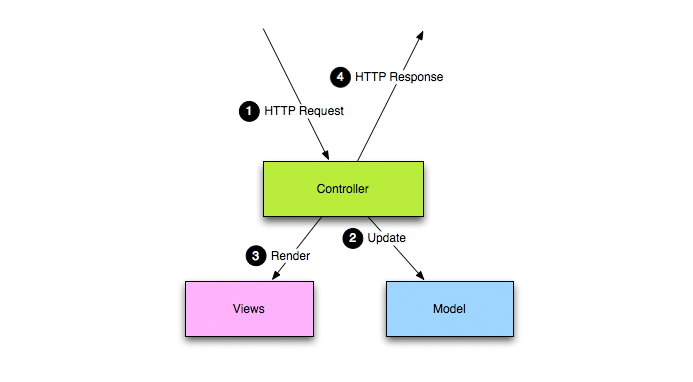
\includegraphics[width=\textwidth]{diagrams_mvc.png}
                \caption{Diagramme MVC}
                \label{fig:Diagramme MVC}
       
\end{figure}
\begin{itemize}
\item Model : Le modèle est la représentation spécifique au domaine de l'information sur laquelle l'application fonctionne. La logique de domaine ajoute «sens» aux données brutes (par exemple : le calcul des totaux, taxes de l'utilisateur, les frais d'expédition pour un panier ...). La plupart des applications utilisent un mécanisme de stockage persistant comme une base de données pour stocker des données. MVC ne mentionne pas spécifiquement la couche d'accès aux données, car il est entendu d'être en dessous, ou encapsulé par le modèle.
\item View : La vue Rend le modèle dans une forme appropriée pour les interactions, en général une interface utilisateur. Plusieurs views peuvent exister pour un modèle unique, à des fins différentes. Dans une application Web, la vue est généralement rendue dans un «format Web» comme HTML, XML ou JSON. Cependant, il existe certains cas où la vue peut être exprimée sous une forme binaire, par exemple rendu dynamique des organigrammes.
\item Controller : Le contrôleur répond aux événements (généralement des actions de l'utilisateur) et les traite, et peut également invoquer des changements sur le modèle. Dans une application Web, les événements sont généralement des requêtes HTTP: un contrôleur écoute les requêtes HTTP, extrait les données pertinentes de la «événement», telles que les paramètres de chaîne de requête, demander des têtes ... Et applique les modifications sur les objets du modèle sous-jacent.

\end{itemize}

\textit{Dans une application play les trois couches sont définies dans un répertoire app, chacun dans un package, ainsi que d'aures package dans le projet Stample comme event, api, services, repository, plugins...}
\newline
\subsection{Cycle de vie d'une requête}
Le framework play est entièrement stateless et orientée Request/Response. Tout les requête HTTP suivent le même path.
\begin{enumerate}
\item Une requête HTTP reçue par le framework.
\item Le Router Component essaie de trouver la route la plus spécifique en mesure d'accepter cette demande. Pour invoker la méthode d'action correspendante. 
\item Le code d'application est executée
\item Si une vue complexe doit être généré, un fichier template est rendu.
\item Le résultat de la méthode d'action (Code de réponse HTTP, Content) s'écrit alors comme une réponse HTTP.
\end{enumerate}


\begin{figure}[H]
        \centering
                \centering
                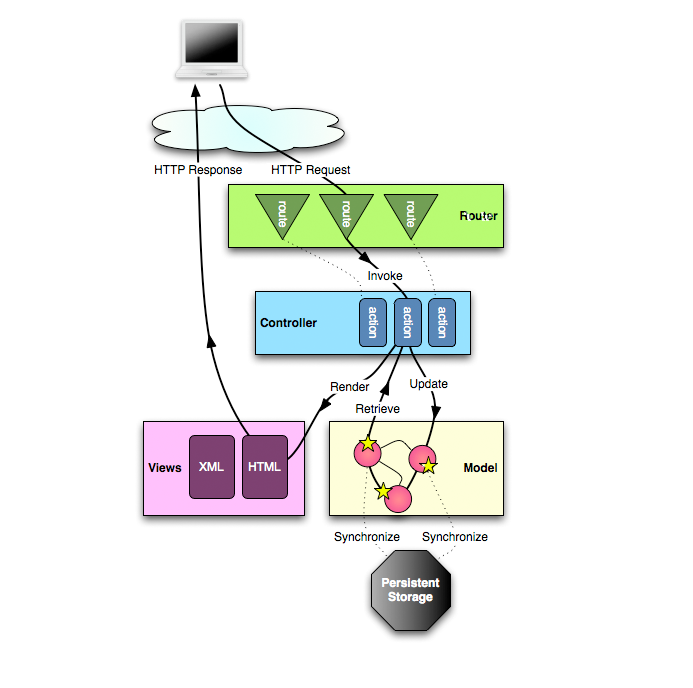
\includegraphics[width=\textwidth]{diagrams_path.png}
                \caption{Diagramme HTTP request path}
                \label{fig:Diagramme HTTP request path}
       
\end{figure}
\newpage
\section{Présentation du contexte Business}
\subsection{Login Antécédent}
Dans la version précedente, il s'agit d'un formulaire classique à remplir pour créer un nouveau compte utilisateur qui sera stocker dans la base mongo avec les coordonnées nécessaires (firstname, fullname, username, passeword, secretCode).
Cela est une première approche, comme la plateforme est en cours de construction des nouveaux besoins apparaissent au fur et à mesure.
Pour plusieurs raisons : Satisfaire la clientèle (utilisateurs de Stample), faciliter la perception de l'interraction et offrir des nouvelles fonctionnalitées classique mais indisponsable.  
\subsection{Critiques}
Cette approche pour la gestion de la création d'un compte utilisateur sur Stample doit être refactoriser.
Il nous manque l'envoi des emails d'information lors des diffèrents étapes d'inscription notament le reset du mot de passe, ainsi que la possibilité de créer un compte à partir d'une autres plateformes en mesure que l'utilisateur s'ennui de reprendre tout un formulaire pour créer un nouveau compte sur une nouvelle plateforme.
\subsection{Fonctionalités manquantes}
\subsubsection{Envoi des mails}
Les utilisateurs de la platefome doivent être notifier par mail lors de l'inscription, l'activation du compte et le changement du mot de passe. 
Les diffèrents emails nécessaires sont signupEmail, welcomeEmail, alreadyRegistredEmail, unknownNotice, passwordResetEmail, passwordChangeNotice.
\subsubsection{Authentification avec d'autres plateformes}
Plusieurs sites web offrent à leurs utilisateurs la possibilité d'utiliser gmail, facebook, twitter ou autres pour le signup.
Cette fonctionnalités facilite l'inscription et rendre cette tâche rapide pour certain utilisateurs.
\subsubsection{Rest mot de passe}
Plusieurs utilisateurs, changent leurs mot de passe d'un site à un autre ce qui provoque souvent l'oublie du cléf.
La gestions des mots de passes oublier est parmis les fonctionnalités indisponsable sur une plateforme.
\subsubsection{AuthCode}
La version Beta de Stample est protégée avec un code d'autorisation, c'est une pratique habituelle pour sécuriser une plateforme mise en ligne et en cours de construction.
\section{Première approche}
\subsection{Etude du modéle}

Après quelques jours pour faire des considérations de conceptions et de mieux comprendre SecureSocial, j'ai réalisé que la mise en œuvre des méthodes n'était pas difficile à comprendre. C'est bien la conception de la logique dans un service backend qui compte. 
SecureSocial offre des APIs (Application Programming Interface) Scala et Java, on utilise ce module Scala pour le Backend de la plateforme.
Ce module open source conçu et développé par Jorge Aliss sous une licence Apache v2.0 disponible sur \textit{GuitHub SecureSocial}\footnote{https://github.com/jaliss/securesocial}. 
Les services d'authentifications sur le soutien de la catégorie des services de premiers plans comme Google, Twitter, Facebook ect..., Il offre aussi un mécanisme de username/password avec les fonctionnaliées Signup, Login, Rest Password.
Ce module support les versions de Play 2.1.x, 2.0.x et 1.x, il est relativement rapide à intégrer dans une application en suivant les instructions sur \textit{le site}\footnote{http://securesocial.ws/guide/getting-started.html}.
SecureSocial est extensible, il est basé sur un modèle d'architecture qui vous permet d'ajouter des nouveaux services d'authentifications.
\newline
\textbf{Utilisation de SecureSocial :}
\textit{carambla} \footnote{http://carambla.com/} : Une application Apple/Android pour chercher, payer ... un parking.
\textit{wimha} \footnote{http://www.wimha.com/} : Un service qui vous permet de proposer et de découvrir des intérêts dans différentes villes du monde.
\textit{webservices} \footnote{https://webservices.io/} : Webservices pour la conversion de documents et fusion de documents...

\subsection{Première Solution}
Les étapes d'implémentation: 
\begin{itemize}
\item J'ai ajouté une nouvelle table dans la base de donnée Stample pour mettre le hash (email, random number, time ),
\item Envoyer le mail avec un lien url?hash=hach,
\item Enfin verifier d'existance du hash dans la base puis faire un sort.

\end{itemize}
 

\section{Remise à Zéro}
Jonathan Winandy est venu joindre l'équipe Stample.
J'ai beaucoup appris aussi de Jonathan qui travaille maintenant à Viadeo et en temps partielle pour Stample.

\subsection{Phase préliminaire}
D'après Jonathan winandy, pour réussir un projet ou une tâche informatique il faut passer par les étapes suivantes :
\begin{itemize}

\item Do It :Commencer par poser le problème et puis écrire du code qui répond a ce besoin.  
\item Do It-Right : Tester le code et l'améliorer.
\item Do It-Fast : Cleaner le code et vérifier les tests.
\end{itemize}
\subsection{Implémentation \& Intégration}

Pour l'intégration de SecureSocial :
\begin{itemize}
\item La vérification de compilation, intégration basique de secure Social dans Stample.
\item Une écriture basique dans la mémoire et l'implémentation de UserService.
\item Working Wiring : Authentification avec email.
\item Ajout du template signUp email.
\item Résoudre les problèmes de Token et de Memory.
\end{itemize}
\subsection{Keep user Logged In SecureSocial :Authenticator Cookie}
Dans le fichier de configuration de SecureSocial il y avait des changements à faire comme la configuration des cookies comme absoluteTimeOutInMinutes(La durée d'authentification d'un utilisateur dans une session. Après cela l'utilisateur doit relogger (par défaut à 720 minutes - 12 heures).
idleTimeoutInMinutes(La durée de session valable depuis la dernière requête (par défaut 30)).
\subsection{Costomisation des templates}
Après l'intégration et la stabilisation des différentes interractions avec le module, j'ai travaillé pour refactoriser les différentes views pour s'adapter avec ce module (le signup, resetPasswordPage, authorisationCode, startResetPassword) et un main global.
En effet, l'authorisationCode c'est un code secret pour protéger la version Beta de Stample(autoriser l'accé qu'à certain utilisateur), il y avait un authorisationCode écrit dans le code de la plateforme que nous avons enlevé pour mettre dans l'interface admin la possibilité de génèrer des diffirents codes d'autorisations.

\subsection{Partie Administrateur sur Stample}
Stample c'est un réseau social en cours de construction il y avait plusieurs bugs et amélioration à ajouter sur la plateforme durant mon stage.
Parmis ces amélioration l'ajout dans l'interface administrateur de l'API la possibilité de génerer/écrire un code
secret pour les utilisateurs l'hors de l'inscription avec un nombre d'usage pour chaque code.
Cela nécessite l'ajout des routes pour gérer et créer les codes d'authentification dans l'admin 
controller et les templates.
J'ai implémenté les différentes templates (authorisationCodes, createCode).
\begin{figure}[htbp]
\begin{minipage}[c]{.5\linewidth}
\begin{center}
\fbox{
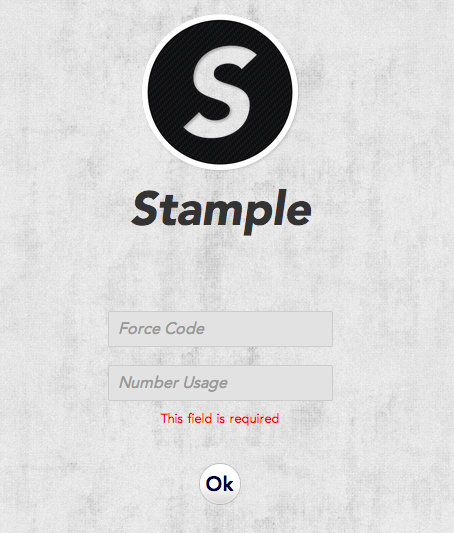
\includegraphics[width=6cm,height=80mm,scale=1]{image1.png}}\hspace{1em}
\caption{Create secret interface}
\label{fig:Create authorisationCode interface}
\end{center}
\end{minipage}
\hfill
\begin{minipage}[c]{.5\linewidth}
\begin{center}
\fbox{
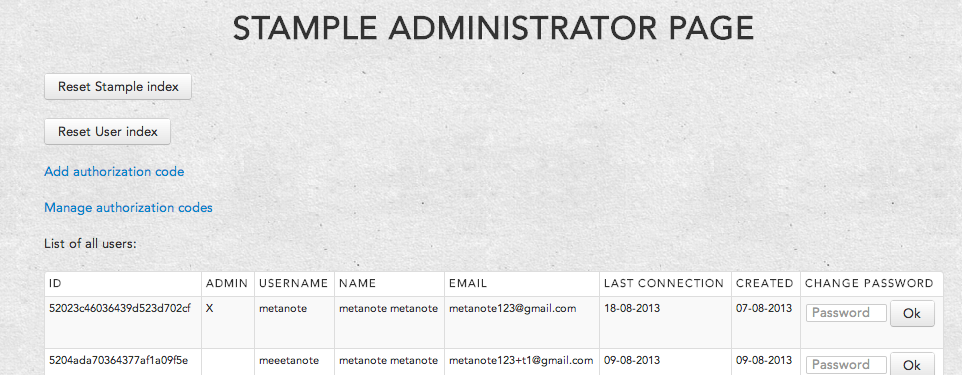
\includegraphics[width=6cm,height=80mm,scale=1]{image2.png}}
\caption{Admin page}
\label{fig:Admin page}
\end{center}
\end{minipage}
\end{figure}

\section{Conclusion}
Cette partie d'authentification sur Stample m'a beaucoup apporté en écrivant du code/des templates et en fixant des bugs.
Sur Backend, l'interaction des controllers, les models et les views avec les différentes classes et traits qui existant déjà m'avait beaucoup aider à comprendre le langage en ajoutant du code compatible avec ce qui existe.
Cette partie du développement m'a permis de reconnaitre le plugin SecureSocial qui peut servir dans d'autres projets et d'améliorer mes connaissances. 

\end{document}